%   % !TEX root = ../../VIII,3_Rahmen-TeX_8-1.tex
%
%
%   Band VIII, 3 N.~??A17.1
%   Signatur/Tex-Datei: LH_35_14_02_048
%   RK-Nr. 58243
%   Überschrift: [Notitia de vi absoluta]
%   Datierung: [Januar 1690]
%   WZ: LEd8-WZ 803012 = RK-WZ 42e / 409 / 767 (ein Fragment) ((gleiches WZ wie in LSB I, 5 N.~275-277))
%   SZ: (keins)
%   Bilddateien (PDF): LH_35_14_02_048_d1; LH_35_14_02_048_d2 (insgesamt zwei)
%
%
\selectlanguage{ngerman}%
\frenchspacing%
%
\begin{ledgroupsized}[r]{120mm}
\footnotesize
\pstart
\noindent\textbf{Überlieferung:}
\pend
\end{ledgroupsized}
\begin{ledgroupsized}[r]{114mm}
\footnotesize
\pstart \parindent -6mm
\makebox[6mm][l]{\textit{L}}%
Notiz: LH~XXXV~14,~2 Bl.~48.
Ein Zettel (9,3 x 9,9 cm);
Fragment eines Wasserzeichens:
italienisches Papier.
Eineinhalb Seiten.
Unlesbar gestrichener Text in der siebten und achten Zeile von Bl.~48~r\textsuperscript{o}.
\pend
\end{ledgroupsized}
%
\selectlanguage{latin}%
\frenchspacing%
%
%
\count\Bfootins=1100
\count\Afootins=1100
\count\Cfootins=1100
%
\vspace{8mm}
\pstart%
\normalsize%
\noindent%
%
\lbrack48~r\textsuperscript{o}\rbrack\ % Blatt 48r
%
\pend%
\vspace{0.5em}
%
  \centerline{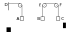
\includegraphics[width=0.43\textwidth]{gesamttex/edit_VIII,3/images/LH_35_14_02_048_d1.pdf}}%
  \vspace{0.5em}
  \centerline{\lbrack\textit{Fig.~1}\rbrack}%
    \vspace{1.5em}%
 % \vspace*{1.0em}%
%  \newpage
%
\pstart%
\noindent%
Dn. Boccabadatus\protect\index{Namensregister}{\textso{Boccabadati} (Boccabadatus), Giovan Battista 1635\textendash1696}
putat, pondus \textit{A} tendens\protect\index{Sachverzeichnis}{pondus tendens}
chordam\protect\index{Sachverzeichnis}{chorda tensa} aequale esse ponderi \textit{B} vel ponderi \textit{C} aequalibus,
chordam tantundem tendentibus,
quia,
pondere \textit{A} subeunte vicem ponderis \textit{C},
ipse paries\protect\index{Sachverzeichnis}{paries} subeat vicem
\edtext{ponderis \textit{B}.\protect\index{Sachverzeichnis}{pondus tendens}
Idque ita a me demonstratur\lbrack:\rbrack}{%
\lemma{ponderis}\Bfootnote{%
\hspace{-0,5mm}\textit{B}.
\textit{(1)}~\textlangle Ego \textendash\ \textendash\ tensio, \textendash\ \textendash\ quod tubus et \textendash\ \textendash\ sent\textendash\textrangle\
\textit{(2)}~Idque ita
\textbar~a me \textit{erg.}~%
\textbar\ demonstratur%
~\textit{L}}}
rigidescat portio chordae,\protect\index{Sachverzeichnis}{chorda tensa} \textit{EF},
manifestum est nihil inde mutari tensionem\protect\index{Sachverzeichnis}{tensio chordae}
manentibus ponderibus \textit{B} et \textit{C}.\protect\index{Sachverzeichnis}{pondus tendens}
Jam \textit{EF} pro pariete\protect\index{Sachverzeichnis}{paries} haberi potest,
et nihil refert quae sit longitudo chordae.
Tantundem igitur chordam\protect\index{Sachverzeichnis}{chorda tensa}
\edtext{tendit pondus \textit{B}}{%
\lemma{tendit}\Bfootnote{%
\textit{(1)}~vis \textit{B}, e
\textit{(2)}~pondus \textit{B}%
~\textit{L}}}
solum\lbrack,\rbrack\
quantum pondera\protect\index{Sachverzeichnis}{pondus tendens} \textit{B} et \textit{C} aequalia
nitentia in contrarias partes.
Quod elegans est paradoxum.\protect\index{Sachverzeichnis}{paradoxon elegans}
Sed hinc non sequitur quod
%\edtext{
ille\protect\index{Namensregister}{\textso{Boccabadati} (Boccabadatus), Giovan Battista 1635\textendash1696}
concludit% }{%
% \lemma{ille concludit}\Cfootnote{%
% Leibniz spielt wohl auf G.\,B. Boccabadatis unveröffentlichte Abhandlung \cite{01237}\textit{De conatu mechanico} an, die in N.~??A17\textsubscript{2} (
% S.~\refpassage{LH_35_10_17_005r+007r_conmech-1}{LH_35_10_17_005r+007r_conmech-2}) genannt wird.}}%
\lbrack,\rbrack\
aequalem esse chordae tensae vim\protect\index{Sachverzeichnis}{vis chordae tensae} duplo
\edtext{\lbrack ponderi\rbrack}{\lemma{pondere}\Bfootnote{\textit{L~ändert Hrsg.}}}
%
a quo tenditur\protect\index{Sachverzeichnis}{pondus tendens}%
\lbrack;\rbrack\
nam, si pro chorda\protect\index{Sachverzeichnis}{chorda tensa}
fingamus liquidum tendibile\protect\index{Sachverzeichnis}{liquidum tendibile}
posset per diversos embolos,\protect\index{Sachverzeichnis}{embolus}
a diversis \makebox[1.0\textwidth][s]{ponderibus\protect\index{Sachverzeichnis}{pondus tendens}
%
\lbrack48~v\textsuperscript{o}\rbrack\ % Blatt 48v
%
simul
\edtext{\lbrack tendi\rbrack,}{%
\lemma{tendit}\Bfootnote{\textit{L~ändert Hrsg.}}}
nec ideo minus tendet
\edtext{unum \lbrack quam\rbrack\ plura,}{%
\lemma{unum}\Bfootnote{%
\textit{(1)}~quantum aliud
\textit{(2)}~\textbar~quantum \textit{ändert Hrsg.}~\textbar\ plura,%
~\textit{L}}}
ob eandem}
\pend
 \vspace{2.0em}%
%
  \centerline{\includegraphics[width=0.21\textwidth]{gesamttex/edit_VIII,3/images/LH_35_14_02_048_d2.pdf}}%
  \vspace{0.5em}
  \centerline{\lbrack\textit{Fig.~2}\rbrack}
\newpage
\pstart
\noindent%
 rationem. Igitur idem dicendum de compressione.\protect\index{Sachverzeichnis}{compressio}
Nec magis aer\protect\index{Sachverzeichnis}{aer compressus} in \textit{AB}
comprimetur a pondere \textit{AC}\protect\index{Sachverzeichnis}{pondus comprimens}
clauso foramine \textit{B},\protect\index{Sachverzeichnis}{foramen}
quam a ponderibus \textit{AC} et \textit{BD} simul.
Et idem est si pluribus adhibitis exitibus\protect\index{Sachverzeichnis}{exitus}
plura adhuc pondera\protect\index{Sachverzeichnis}{pondus comprimens} adhibeantur%
\lbrack;\rbrack\
tantum enim unum facit quantum infinita.
\pend%
%
%% \newpage
% \vspace{1.5em}%
%%
%  \centerline{\includegraphics[width=0.21\textwidth]{gesamttex/edit_VIII,3/images/LH_35_14_02_048_d2.pdf}}%
%  \vspace*{0.5em}
%  \centerline{\lbrack\textit{Fig.~2}\rbrack}%
  \newpage%
  \count\Bfootins=1200
\count\Afootins=1200
\count\Cfootins=1200
%
%
% ENDE DES STÜCKES auf Blatt 48v
%
% \vspace*{-1.0em}%    REIN VORLÄUFIG   !!!!
%